\chapter{Wifi Direct}
\label{cha:WifiDirect}
This chapter gives a short overview over Wifi Direct. Everything not mentioned or details about Wifi Direct can be found in the article "Wi-Fi CERTIFIED Wi-Fi Direct" from the Wi-Fi Alliance\cite{wifialliance}.

\section{Overview}
\label{sec:Overview}
Wi-Fi Direct, or sometimes simply Wi-Fi P2P, is a standard which allows devices to connect directly to each other without requiring a wireless access point. With this technology users can connect to other devices in a way that makes it simpler and convenient for them. Because of the ability to connect directly to other Wi-Fi Direct devices, smartphones, printers, PCs and gaming devices can share their services without accessing a traditional network. Instead of connecting first to an existing infrastructure network and then connecting to another device, users can so directly connect to the device which offers the services they need. Wi-Fi Direct devices are allowed to create a one-to-one connection, or they could form a group with several devices.
Wi-Fi Direct devices support also the possibility to establish a connection with existing legacy Wi-Fi devices. This offers the possibility to create a direct connection with the hundreds of millions legacy Wi-Fi certified devices (802.11 a/g/n). According to documentation of the Wi-Fi Alliance paper the usage of Wi-Fi Direct brings some benefits for their users, among these:\\
\begin{description}
  \item[Mobility and Portability:] \hfill \\ Wi-Fi Direct devices can connect anytime and everywhere, because a Wi-Fi router or an access point is not required.
  \item[Immediate Utility:] \hfill \\ Once the user buys his first Wi-Fi Direct device, he is immediately able to create a direct connection between devices. Even if it is his first Wi-Fi Direct device at home, he could establish a direct connection with his existing legacy Wi-Fi devices.
  \item[Ease of Use:] \hfill \\ The ability of Wi-Fi Direct discovery and the Service discovery allow users to find and identify available devices and services before establishing a connection.
  \item[Simple Secure Connection:] \hfill \\ Devices with Wi-Fi direct use Wi-Fi Protected Setup (WPS) which allows to simple create a secure connection. To establish a secure connection the user has to press a button on both devices, or type in a Pin. The procedure depends on the device type\\
\end{description}

\noindent At the present time\footnote{\label{foot:1}June 2014.} there are four Wi-Fi Direct standard generations. Devices that are equipped with the latest 802.11n Wi-Fi Direct standard, must be backwards compatible and must be able to communicate with devices which adapts older standards. The table below gives an overview of the current standards:

\begin{center}
	\begin{table}[h]
    	\begin{tabular}{| l | l | p{6cm} |}
    	\hline
    	Standard & Bandwidth & Range\\ \hline
		Wi-Fi Direct 802.11.a & 54 Mbps & 10 meters \\ \hline
		Wi-Fi Direct 802.11.b & 11 Mbps & 20-50 meters inside buildings. \newline
		Up to 500 meters outside\\ \hline
		Wi-Fi Direct 802.11.g & 54 Mbps & 90 meters inside buildings. \newline
		Up to 400 meters outside\\ \hline
		Wi-Fi Direct 802.11.n & 450 Mbps & 150 meters inside building.\newline
		Up to 500 meters outside\\ \hline
    	\end{tabular}
    \caption{Overview of the Wi-Fi Direct standards }
    \label{table:Wi-Fi Direct}
    \end{table}
\end{center}
\noindent The data in the table were taken from the official Wi-Fi Direct standards there is no guarantee that all Wi-Fi Direct devices have to comply with these.
\section{Technology Basics}
\label{sec:TechnologyBascs}
Wi-Fi direct devices are capable of establish a peer-to-peer connection. They can form groups in a one-to-one or one-to-many topology. One Wi-Fi direct device is responsible for the group and acts as group owner. For legacy clients the group owner will appear as an Access Point on which they could connect.
All Wi-Fi direct devices must be able to be in charge of a group and act as group owner. Furthermore all devices must be able to negotiate which device adopts the group owner role when they forming a new group with other Wi-Fi Direct devices. A group can contain Wi-Fi Direct devices and legacy devices, with the limitation that legacy devices can only act as clients within a group. The picture below shows a typical Wi-Fi Direct P2P group.

\begin{figure}[ht]
	\centering
  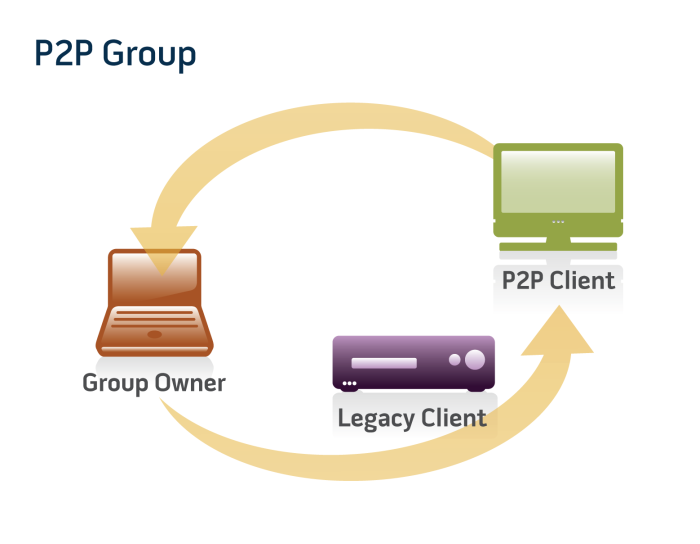
\includegraphics[width=0.7\textwidth]{images/wifidirect.png}
	\caption{The figure shows a P2P group with a Wifi Direct client and a legacy device}
	\label{fig1}
\end{figure}